\documentclass{article}
\usepackage{tikz, comment}
\usepackage{pifont}
\usepackage{fontspec}
\usetikzlibrary{arrows, decorations.markings, decorations.pathreplacing}
\begin{comment}
:Title: Not defined yet
:Tags: slope;rule;functions;figure;curve
:Author: Prof.Hu Ji-shan, HKUST
:Slug: No name yet

Description Here.........
\end{comment}
\begin{document}\centering

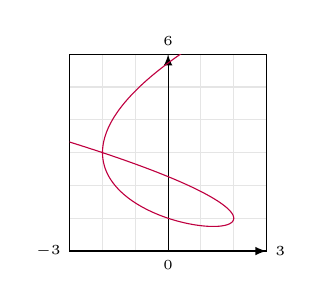
\begin{tikzpicture}[>=latex,xscale=0.25*10/6, yscale=0.25*10/6][font=\sf\small]

\draw[xstep=1cm,ystep=1cm,color=gray!20] (-3, 0) grid (3, 6);

\draw[->] (-3, 0) -- (3, 0);
\draw[->] (0, 0) -- (0, 6);

\node[left] at (-3, 0) {\tiny$-3$};
\node[right] at (3, 0) {\tiny$3$};
\node[below] at (0, 0) {\tiny$0$};
\node[above] at (0, 6) {\tiny$6$};

\clip[draw] (-3, 0) rectangle (3, 6);

\draw[purple, samples=200, smooth, domain=-2.5:2, variable=\t]
plot ({(\t)^3-3*(\t)}, {(\t)^2+\t+1});

\end{tikzpicture}
\end{document}